\documentclass[./main.tex]{subfiles}

\begin{document}
\section{Descrizione dell'analisi}
Modalità di raccolta dati (...).
\\
Sono state calcolate le seguenti variabili di riassunto del segnale:
\begin{itemize}
	\item Integrale del segnale nell'intervallo, calcolato con l'approssimazione per trapezi.
	\item Massimo dell'accelerazione nell'intervallo.
	\item Variazione media assoluta della derivata nell'intervallo.
\end{itemize}
Per condurre una prima analisi esplorativa le tecniche d'analisi utilizzate sono state le seguenti:
\begin{itemize}
	\item PCA sui dati sbiancati.
	\item ICA sui dati sbiancati.
	\item t-SNE.
	\item t-SNE sui dati sbiancati.
\end{itemize}
I risultati ottenuti:
\begin{figure}[H]
	\centering
	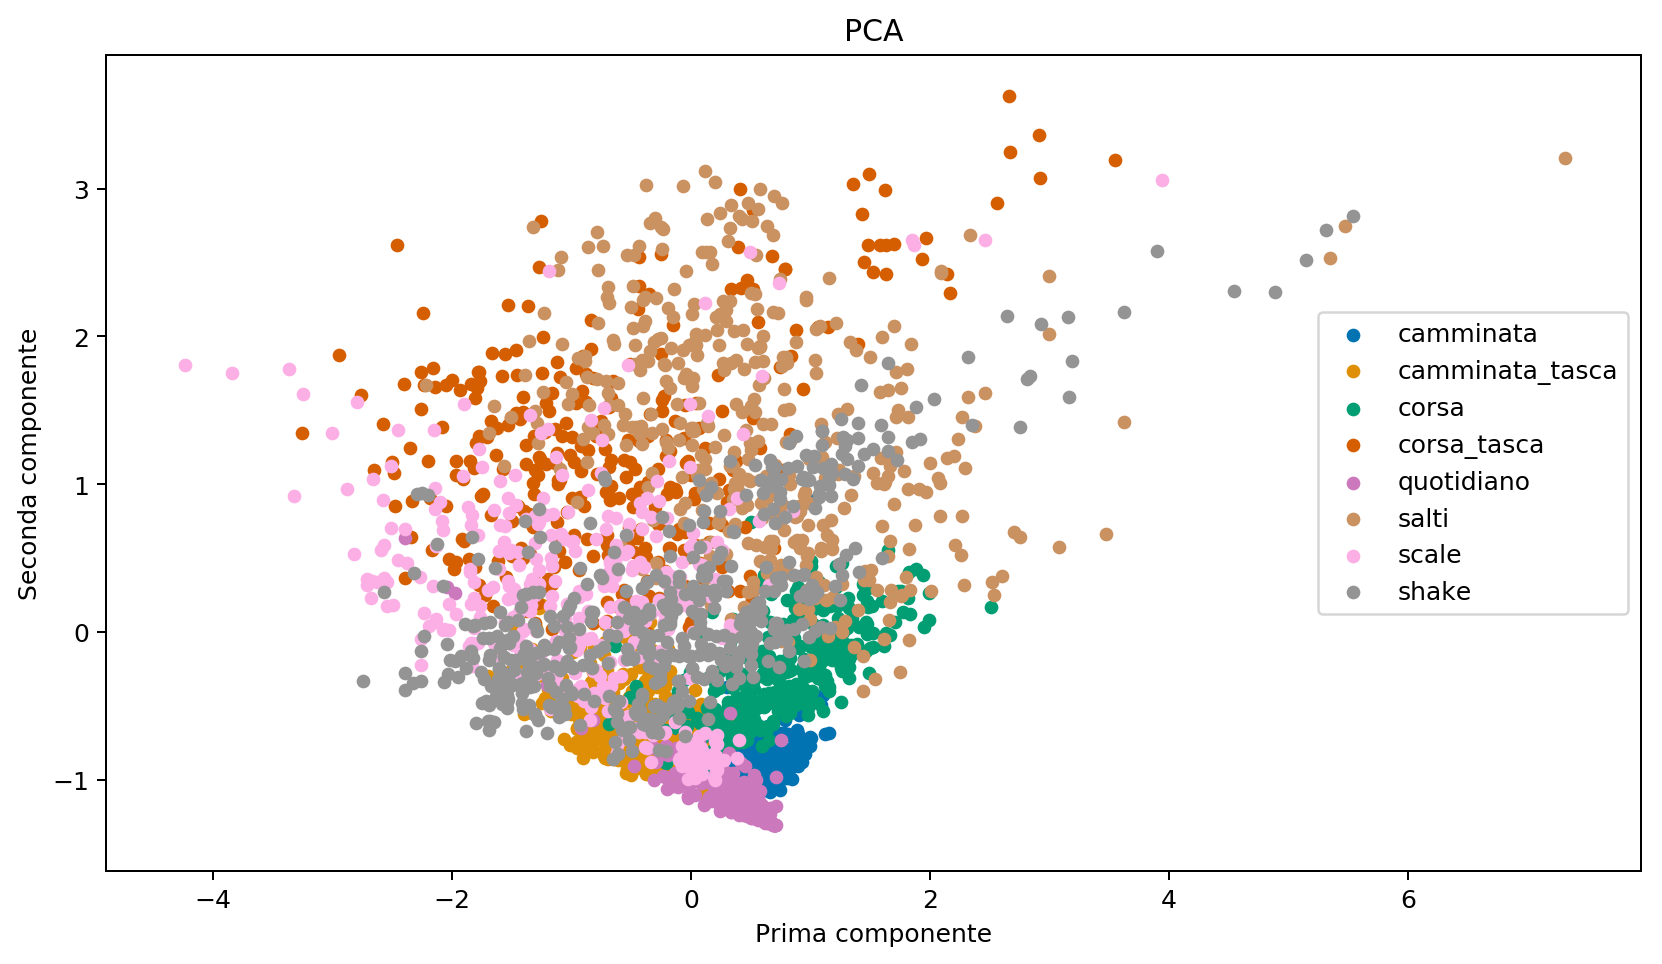
\includegraphics[width=.9\textwidth, height=.9\textheight, keepaspectratio]{../../figure/PCA.png}
	\caption{{ Analisi esplorativa con PCA su dati sbiancati}}
	\label{PCA}
\end{figure}

\begin{figure}[H]
	\centering
	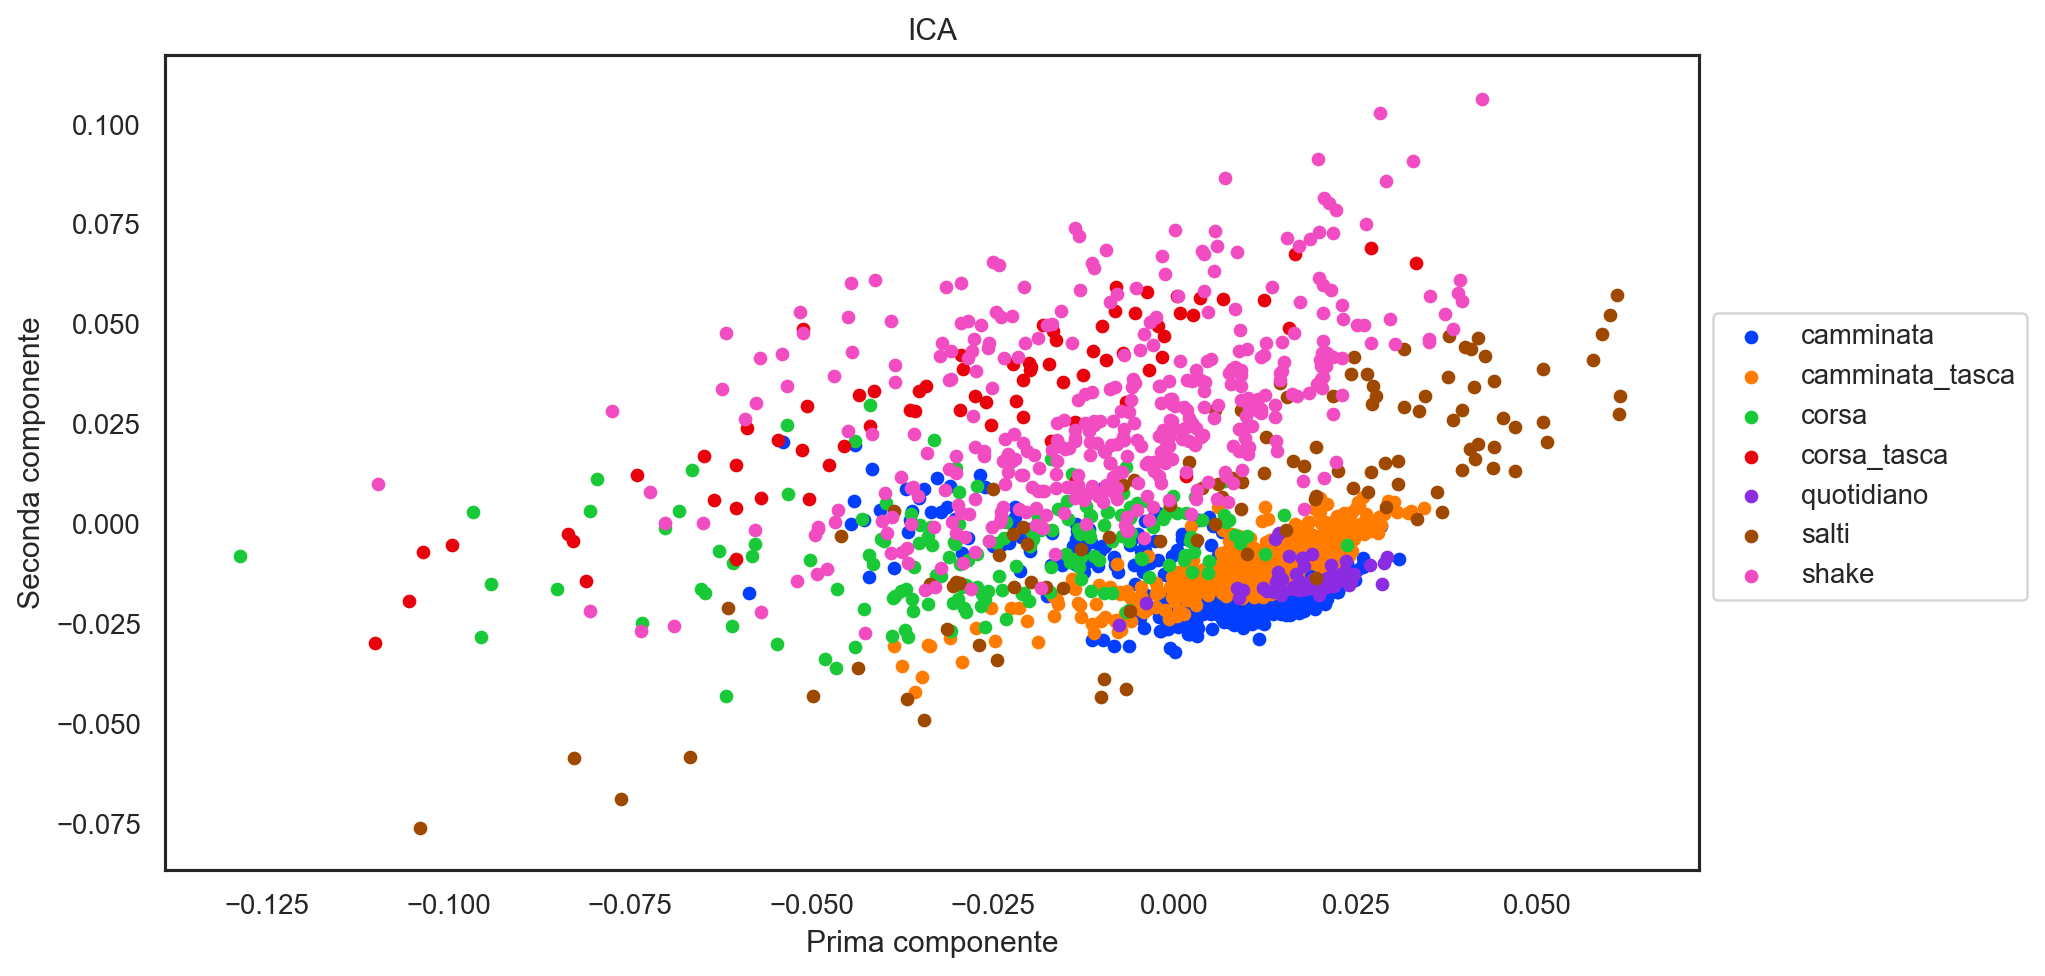
\includegraphics[width=.9\textwidth, height=.9\textheight, keepaspectratio]{../../figure/ICA.png}
	\caption{{ Analisi esplorativa con ICA su dati sbiancati}}
	\label{ICA}
\end{figure}

\begin{figure}[H]
	\centering
	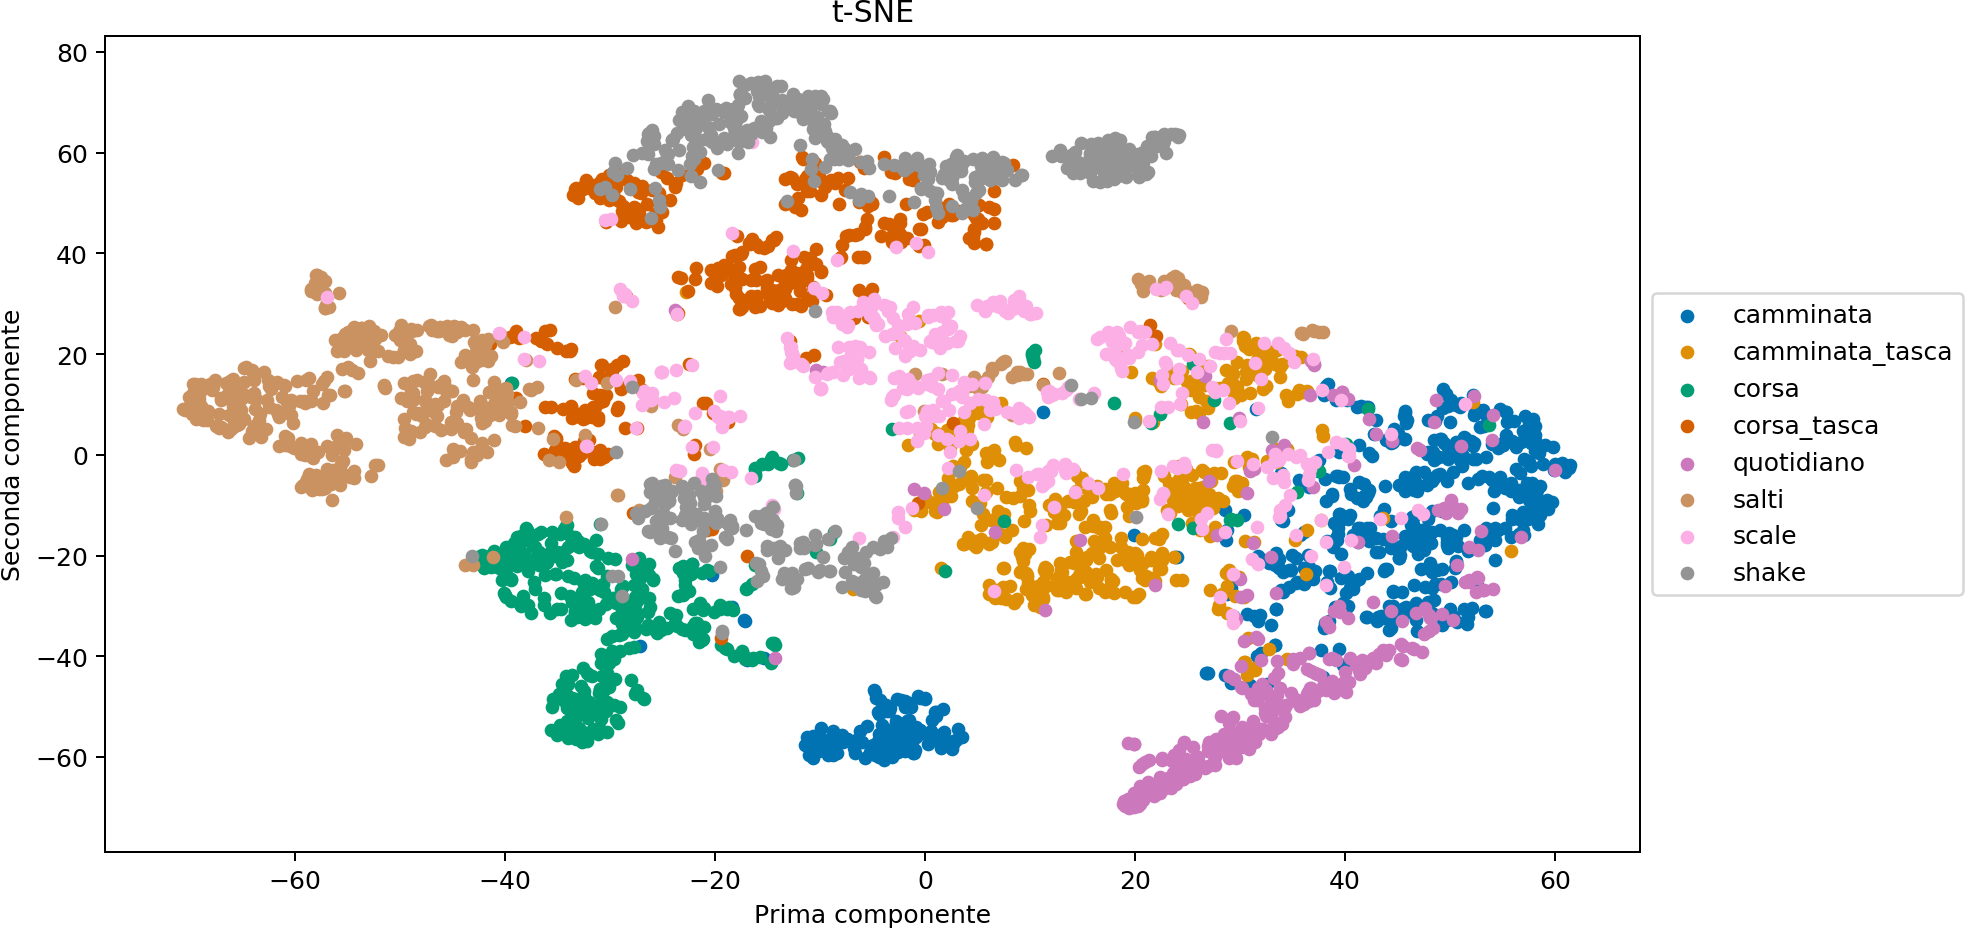
\includegraphics[width=.9\textwidth, height=.9\textheight, keepaspectratio]{../../figure/t-SNE.png}
	\caption{{ Analisi esplorativa con tSNE su dati sbiancati}}
	\label{tSNE}
\end{figure}
Al fine di riuscire a discriminare l'azione svolta, classificata in "camminata", "camminata tasca", "corsa", "corsa tasca", "quotidiano", e "shake", sono stati applicati i seguenti algoritmi di classificazione:
\begin{itemize}
	\item Regressione multinomiale.
	\item Alberi di classificazione.
	\item t-SNE sui dati sbiancati.
\end{itemize}


\end{document}